\chapter{Tecnologie}

%
%
%
\section{Stack MEVN}

L’applicazione è stata sviluppata sulla base dello stack MEVN, che come l’acronimo comprende le seguenti tecnologie:

\begin{itemize}
    \item \textbf{MongoDB}: È il database NoSQL utilizzato come backend per memorizzare i dati. MongoDB è flessibile, scalabile e adatto per la gestione di dati non strutturati o semistrutturati.

    \item \textbf{Express}: È un framework JavaScript per la creazione di server web. Express semplifica la gestione delle richieste HTTP, il routing e \\l'implementazione di middleware nel server.

    \item \textbf{Vue.js}: È un framework JavaScript progressivo per la creazione di interfacce utente. Vue.js è noto per la sua facilità d'uso e offre una solida architettura per lo sviluppo di interfacce utente interattive.

    \item \textbf{Node.js}:è un runtime per l'esecuzione di codice JavaScript.
\end{itemize}

%
%
%
\section{Strumenti, Framework \& Librerie utilizzati}
% Da riscrivere meglio

%
%
%
\subsection{Docker}

Docker è un software progettato per eseguire processi informatici in ambienti isolabili noti come \emph{container}, semplificando la creazione, la distribuzione e l'esecuzione di applicazioni.
%
I container includono il codice dell'applicazione, le librerie e le dipendenze, garantendo che l'applicazione funzioni in modo coerente su qualsiasi ambiente in cui venga eseguita.
%
Le principali caratteristiche di Docker includono:

\begin{enumerate}
    \item \textbf{Isolamento dell'ambiente}: Docker offre un alto grado di isolamento, consentendo alle applicazioni di essere eseguite indipendentemente senza interferire con altre applicazioni sullo stesso sistema.

    \item \textbf{Portabilità}: I contenitori Docker sono altamente portabili. Un contenitore Docker può essere eseguito su qualsiasi sistema che esegua Docker, indipendentemente dal sistema operativo sottostante.

    \item \textbf{Velocità e leggerezza}: I contenitori Docker sono avviati in pochi secondi e richiedono meno risorse rispetto alle macchine virtuali, rendendo Docker ideale per distribuzioni scalabili e veloci.
\end{enumerate}

%
%
%
\subsubsection{Utilizzo}

Docker è stato utilizzato per eseguire il deploy di tutti i componenti del sistema, tra cui:

\begin{itemize}
    \item Webserver per microservizi
    \item Database per microservizi
    \item Servizi di utility
    \item Broker
    \item API Gateway
\end{itemize}

%
%
%
\subsection{Swagger}

Swagger è un insieme di strumenti open source per progettare, creare, documentare e consumare servizi web RESTful, attraverso la specifica \emph{Open API}.
%
L'obiettivo principale di Swagger è semplificare e standardizzare il processo di sviluppo e integrazione di API, fornendo una documentazione interattiva e uno strumento per testare direttamente le API.

Le caratteristiche chiave di Swagger includono:

\begin{itemize}
    \item Definizione della API: Swagger utilizza il formato YAML o JSON per definire la struttura e i dettagli di un'API RESTful, specificando risorse, operazioni, parametri, tipi di dati, e altro ancora.
    
    \item Interfaccia Utente Interattiva: Genera automaticamente un'interfaccia utente interattiva (Swagger UI) basata sulla definizione dell'API. Questa interfaccia consente agli sviluppatori di esplorare e testare le API direttamente dal browser.

    \item Standardizzazione e Conformità: Swagger promuove la standardizzazione nelle API RESTful, migliorando la coerenza e la comprensione tra sviluppatori e team di sviluppo
\end{itemize}

\subsubsection{Utilizzo}

Con Swagger, è stato possibile creare documentazione dettagliata delle API, specificando dettagli come gli endpoint, i parametri, i tipi di dati, le risposte possibili e persino esempi di richieste e risposte.

La documentazione delle API del progetto è consultabile sulle Github Pages:
\url{https://zucchero-sintattico.github.io/piperchat/api/rest/}

%
%
%
\subsection{AsyncApi}

AsyncAPI è uno standard di specifica per la progettazione di API asincrone.
%
Simile a come OpenAPI è utilizzato per definire e documentare API sincrone, AsyncAPI è progettato specificamente per gestire le comunicazioni asincrone, come quelle basate su messaggi o eventi.

Le principali caratteristiche di AsyncAPI includono:

\begin{itemize}
    \item Comunicazioni Asincrone: AsyncAPI è progettato per modellare API che coinvolgono comunicazioni asincrone, dove la richiesta e la risposta non sono sincronizzate nel tempo.

    \item Documentazione Dettagliata: Come OpenAPI per API sincrone, AsyncAPI fornisce una specifica dettagliata per documentare aspetti come endpoint, messaggi, schemi dei dati, protocolli di trasporto e altri dettagli relativi alla comunicazione asincrona.

    \item Supporto per Protocolli Comuni: AsyncAPI supporta una varietà di protocolli comuni per la comunicazione asincrona, come MQTT, AMQP e WebSocket. Ciò consente una flessibilità nella progettazione delle API a seconda delle esigenze specifiche del progetto.
\end{itemize}

%
%
%
\subsubsection{Utilizzo}

AsyncAPI è stato utilizzato come strumento di supporto e di documentazione di tutte le tipologie di messaggi rappresentanti gli eventi che vengono scambiati tramite il broker all'interno dell'architettura a microservizi.

La documentazione delle API per i messaggi infra-servizi è consultabile sulle Github Pages:
\url{https://zucchero-sintattico.github.io/piperchat/api/infra-service/}

Inoltre, la tecnologia è stata sfruttata anche per la documentazione dei messaggi inviati ai client come notifiche di eventi.
Tale documentazione è disponibile al seguente link:
\url{https://zucchero-sintattico.github.io/piperchat/api/notification/}

%
%
%
\subsection{Traefik}

Traefik è un moderno \emph{reverse proxy} e \emph{load balancer} progettato per gestire il traffico web in ambienti complessi e distribuiti.
%
La sua funzione principale è quella di agire come un \emph{API Gateway}, instradando e distribuendo il traffico tra il frontend e i diversi microservizi del backend.

%
%
%
\subsubsection{Utilizzo}

Nel contesto del nostro progetto, l'utilizzo di Traefik è stato implementato in modo agevole e efficiente.
%
All'interno di ciascun file \emph{Docker Compose} relativo ai singoli servizi, abbiamo semplicemente specificato le richieste o le rotte accettate dal microservizio attraverso l'aggiunta di una label.
%
Questo approccio ci ha permesso di configurare facilmente e in modo dettagliato le direttive per il routing del traffico verso ciascun servizio, consentendo a Traefik di instradare le richieste in base alle specifiche esigenze di ciascun microservizio.

Di seguito è riportato un esempio della definizione delle rotte.

\begin{verbatim}
    labels:
      - |
        traefik.http.routers.users-service.rule=
        (Method(`GET`) && Path(`/friends`)) ||
        (Method(`GET`) && Path(`/whoami`)) ...
\end{verbatim}

%
%
%
\subsection{WebRTC}

\emph{WebRTC}, acronimo di "Web Real-Time Communication," è una tecnologia open-source che consente la comunicazione audio e video in tempo reale direttamente tra browser web senza richiedere plugin o software aggiuntivi.
%
È utilizzato per creare applicazioni di videoconferenza, chat video, streaming multimediale e altro.

Le principali caratteristiche di WebRTC includono:

\begin{enumerate}
    \item \textbf{Comunicazione peer-to-peer}: WebRTC consente ai browser di comunicare direttamente tra loro, evitando la necessità di server intermediari per la trasmissione di dati in tempo reale.

    \item \textbf{Supporto per audio e video}: WebRTC supporta la comunicazione audio e video in tempo reale, consentendo agli utenti di interagire tramite chat video o conferenze online.

    \item \textbf{Accesso ai dispositivi}: WebRTC consente l'accesso ai dispositivi hardware come telecamere e microfoni per abilitare la cattura audio e video.
\end{enumerate}

%
%
%
\subsubsection{Utilizzo}

Webrtc è stato utilizzato per la gestione delle video chiamate dei canali multimediali e infra-utente.
%
Questo ha permesso di evitare lo sviluppo di un servizio adibito allo streaming audio e video degli utenti, lasciando tale compito agli utenti stessi in maniera peer-to-peer.

%
%
%
\subsubsection{Funzionamento}

Nel contesto di WebRTC, ci sono tre concetti chiave: \textbf{offer}, \textbf{answer}, e \textbf{ICE candidates}.

\begin{itemize}
    \item \textbf{Offer}:
    L'offerta è il punto di partenza per l'inizializzazione di una connessione WebRTC.

    Un peer (la parte che inizia la connessione) crea un'offerta che specifica le sue preferenze per la sessione di comunicazione, inclusi i codec supportati, i parametri di sicurezza, etc.
    L'offerta è creata utilizzando l'API \textit{createOffer().}

    \item \textbf{Answer}:
    L'answer è generata dal peer destinatario in risposta all'offerta ricevuta.
    
    Il peer destinatario, dopo aver ricevuto l'offerta, crea una risposta che riflette le sue preferenze per la comunicazione.
    L'answer è creata utilizzando l'API \textit{createAnswer().}

    \item \textbf{ICE Candidates}:
    ICE (Interactive Connectivity Establishment) è un protocollo utilizzato per stabilire una connessione in presenza di reti complesse, come dietro firewall o NAT.
    I candidati ICE sono gli indirizzi IP e le porte su cui un peer può essere contattato.
    Durante il processo di offerta e risposta, i peer scambiano i loro candidati ICE utilizzando l'API onicecandidate.
    Il processo di raccolta dei candidati ICE è noto come "ICE gathering".
\end{itemize}

In sintesi, il flusso tipico di inizializzazione di una connessione WebRTC coinvolge la creazione di un'offerta da parte del peer iniziatore, la trasmissione di questa offerta al peer destinatario, la creazione di una risposta da parte del peer destinatario e, infine, lo scambio di candidati ICE per stabilire una connessione diretta tra i due peer.
%
Questo processo è fondamentale per consentire la comunicazione bidirezionale in tempo reale tra browser senza passare attraverso un server intermedio.

%
%
%
\subsubsection{Protocollo per videochiamate basato su eventi}

Per la gestione dello scambio di informazioni necessarie ad instaurare una comunicazione webrtc tra utenti è stato sviluppato un apposito servizio che opera su un protocollo che ha permesso di mettere in contatto tutti i partecipanti di una determinata sessione, in modo da avere un accesso uniforme e un aggiornamento reattivo all'arrivo o all'uscita degli utenti.

\begin{figure}[htbp]
    \centering
    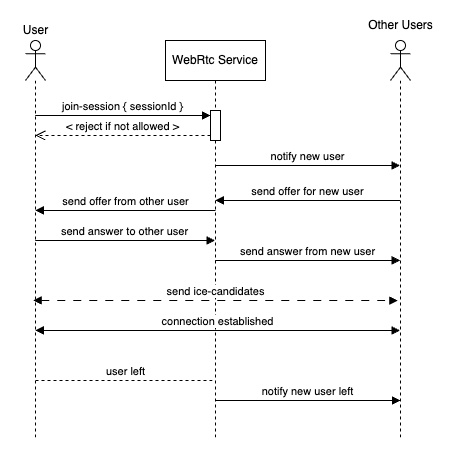
\includegraphics[width=\textwidth]{img/piperchat-WebRTC.drawio.png}
    \caption{Protocollo chiamate webrtc}
    \label{fig:webrtc-protocol}
\end{figure}

%
%
%
\subsection{SocketIO}

Socket.IO è una libreria JavaScript che fornisce una comunicazione bidirezionale in tempo reale tra il server e il client in applicazioni web.
%
È spesso utilizzata per implementare funzionalità di chat, giochi multiplayer, aggiornamenti in tempo reale e altre applicazioni che richiedono una comunicazione immediata tra il server e il browser.
%
Le principali caratteristiche di Socket.IO includono:

\begin{enumerate}
    \item \textbf{Comunicazione in tempo reale}: Socket.IO consente una comunicazione bidirezionale in tempo reale, consentendo agli utenti di ricevere aggiornamenti istantanei dal server.

    \item \textbf{Supporto multipiattaforma}: Socket.IO è compatibile con diverse piattaforme e browser, consentendo una comunicazione uniforme su molteplici dispositivi.

    \item \textbf{Messaggi personalizzati}: Gli sviluppatori possono definire messaggi personalizzati per gestire eventi specifici nell'applicazione, come messaggi di chat o aggiornamenti di gioco.

    \item \textbf{Riconnessione automatica}: Socket.IO supporta la riconnessione automatica in caso di perdita di connessione, garantendo che gli utenti rimangano connessi.

    \item \textbf{Ampia adozione}: Socket.IO è ampiamente utilizzato nella comunità di sviluppatori ed è supportato da molte piattaforme e framework.

\end{enumerate}

%
%
%
\subsubsection{Utilizzo}

Socket.io è stato utilizzato per sviluppare i sistemi di comunicazione con i microservizi che richiedevano un aggiornamento continuo di informazioni o uno scambio di dati reciproco.

In particolare è stato implementato nei seguenti sistemi:

\begin{itemize}
    \item Sistema di notifiche: poiché era necessaria un elevata reattività e una continua connessione al server da parte degli utenti per ricevere le notifiche.

    \item Gestione dello status online degli utenti.
    
    \item Sistema di videochiamate: sfruttato per la gestione del protocollo per l'accesso a videochiamate e per tutti gli aggiornamenti che ne conseguono come join e left di un utente.
\end{itemize}

%
%
%
\subsection{Quasar}

Quasar Framework è un framework open-source basato su Vue.js, progettato per semplificare lo sviluppo di applicazioni web e mobile con un unico codice sorgente.
%
È noto per la sua flessibilità e la capacità di generare applicazioni per diverse piattaforme.
%
Le caratteristiche principali di Quasar Framework includono:

\begin{enumerate}
    \item \textbf{Componenti Vue.js predefiniti}: Quasar offre una vasta libreria di componenti Vue.js personalizzati e ricchi di funzionalità, che semplificano la creazione di interfacce utente sofisticate.

    \item \textbf{Responsive Design}: Le applicazioni Quasar possono essere facilmente rese responsive per adattarsi a diversi dispositivi e dimensioni dello schermo.

    \item \textbf{Material Design}: Quasar aderisce a Material Design di Google, offrendo un aspetto moderno e uniforme per le applicazioni.
\end{enumerate}

%
%
%
\subsubsection{Utilizzo}

Quasar è stato impiegato per i componenti principali dell'interfaccia utente che il framework offre.

%
%
%
\subsection{Pinia}

Pinia JS è una libreria di gestione dello stato progettata per applicazioni Vue.js.
%
Essa fornisce un'architettura di gestione dello stato centralizzata e reattiva, offrendo uno store centralizzato per memorizzare e gestire lo stato dell'applicazione.
%
Pinia si basa sui concetti principali di Vue.js, come la reattività e la gestione delle modifiche dello stato in modo efficiente.
%
Questo strumento consente agli sviluppatori di scrivere codice pulito e manutenibile, facilitando la gestione dello stato dell'applicazione Vue.js.

%
%
%
\subsubsection{Utilizzo}

Nella nostra applicazione Vue, lo stato globale è stato gestito tramite la definizione di svariati store.
%
Ogni store è stato progettato per occuparsi di specifici aspetti funzionali dell'applicazione, fornendo una struttura chiara e distintiva per la gestione dei dati.

Sono stati definiti i seguenti store:

\begin{itemize}
    \item \textbf{Store `app':} Gestisce le informazioni globali dell'applicazione.
    
    \item \textbf{Store `friend':} Si occupa della gestione delle informazioni relative agli amici all'interno dell'applicazione.
    
    \item \textbf{Store `messages':} Gestisce la logica e i dati relativi ai messaggi.

    \item \textbf{Store `photo':} Gestisce il salvataggio e la fruizione delle foto all'interno dell'applicazione, in particolare è stato usato per fare caching delle foto degli utenti.

    \item \textbf{Store `users-status':} Gestisce le informazioni relativo allo stato degli utenti (online/offile/ultimo accesso) tramite un sistema di caching che ne permette la fruizione in modo semplice.
    
    \item \textbf{Store `monitoring':} Si occupa della raccolta e visualizzazione dei dati relativi al monitoraggio dei microservizi dell'applicazione.
    
    \item \textbf{Store `notifications':} Gestisce le notifiche dell'applicazione, inclusi avvisi, notifiche push e loro gestione.
    
    \item \textbf{Store `server':} Gestisce le comunicazioni relative ai server e ai canali.
    
    \item \textbf{Store `user':} Si occupa delle informazioni e delle azioni relative all'utente, inclusi i dati del profilo e le operazioni di autenticazione.
    
    \item \textbf{Store `webrtc':} Gestisce le funzionalità e lo stato relativi alle comunicazioni in tempo reale tramite WebRTC, inclusi audio, video e connettività.
\end{itemize}

%
%
%
\section{Linguaggi}

I linguaggi di programmazione utilizzati all'interno del progetto sono i seguenti:

\begin{itemize}
    \item \textbf{Typescript}: sia per il backend che per il frontend

    \item \textbf{HTML}: per la realizzazione delle web pages

    \item \textbf{CSS}: per i fogli di stile 
\end{itemize}
